\documentclass[14px]{article}
\usepackage{xeCJK}
\usepackage[frenchb]{babel}
\usepackage[T1]{fontenc}
\usepackage[utf8]{inputenc}
\usepackage{textcomp}
\usepackage{amssymb}
\usepackage[ruled,longend]{algorithm2e}
\usepackage{amsmath}
\usepackage{latexsym}
\usepackage{fancyhdr}
\usepackage{geometry}
\usepackage{setspace}
\usepackage[colorlinks,linkcolor=blue]{hyperref}
% Image
\usepackage{graphicx}
\usepackage{float}
\usepackage{subfigure}
\usepackage{enumerate}

\begin{document}
	
	\setlength{\parindent}{0pt}
	\begin{titlepage}
		\begin{center}
			% Upper part of the page
			
\includegraphics[width=0.35\textwidth]{logo.png}\\[1cm]
			\textsc{\Large Rapport de PSTL}\\[0.5cm]
			% Title
			{ \huge \bfseries Simulateur \& IDE génériques pour OMicrob}\\[0.4cm]
			% Author and supervisor
			\begin{minipage}{0.4\textwidth}
				\begin{flushleft} \large
					\emph{Author:}\\
					Qiwei \textsc{XIAN}\\
					Ruiwen \textsc{WANG}\\
				\end{flushleft}
			\end{minipage}
			\begin{minipage}{0.4\textwidth}
				\begin{flushright} \large
					\emph{Professeur:} \\
					Prof.\textsc{Emmanuel Chailloux}
				\end{flushright}
			\end{minipage}
			\vfill
			% Bottom of the page
			{\large \today}
		\end{center}
		
	\end{titlepage}
	\clearpage
	
	\tableofcontents
	\thispagestyle{empty}
	\clearpage
	
	\pagestyle{fancy}
	\lhead{Introduction}
	\rhead{\thepage}
	\fancyfoot{}
	
	
	\section{Introduction}
	
	\subsection{Microcontrôleur}
	Microcontrôleur est un circuit intégré largement utilisé dans les systèmes embarqués, ils consistent aux CPU, mémoire, minuterie/compteur, divers ports d'entrée et de sortie. Son plus grand avantage est sa petite taille, donc qui peut être placée à l'intérieur des dispositifs. Mais aussi ils sont soumis à des contraintes de taille, il a une petite capacité de stockage, des interfaces d'entrée et de sortie très simples et ils n'ont parfois aucun dispositif d'interface homme-machine : ni clavier, ni écran, etc. Limité par sa capacité de stockage et CPU, les programmeurs ne peuvent utiliser que des langages de bas niveau tels que le langage C et le langage d'assemblage pour la programmation, et ils ne peuvent pas utiliser de langages de programmation de haut niveau tels que JAVA et OCaml, ce qui entraîne des difficultés de développement pour les programmeurs. Nous pouvons utiliser OmciroB pour convertir le fichier OCaml en un fichier hexadécimal qui peut être exécuté dans le microcontrôleur. Néanmoins, puisque la fonction d'affichage du microcontrôleur est limitée, afin de comprendre le processus d'exécution du programme et de faciliter le débogage du programme, nous avons besoin d'un simulateur pour simuler le comportement du microcontrôleur lors de l'exécution du programme sur le PC.
	\subsection{OmicroB}
	OMicroB est une machine virtuelle OCaml écrite directement en langage C, il dédie à l'exécution de programmes OCaml sur microcontrôleur avec des ressources très limitées.
	
	\subsubsection{Structure de OmicroB}
	Notre objectif de projet : le simulateur pour simuler le comportement du microcontrôleur lors de la génération de fichiers depuis OmicroB, donc il sera implémenté sur la base d'OmicroB. Il faut donc d'abord comprendre comment cela marche à partir de structure d'OmicroB.\\
	
	\clearpage
	
	\begin{figure}
		\subfigure[Le structure de OmicroB]{
			\begin{minipage}[t]{\linewidth}
				\centering
				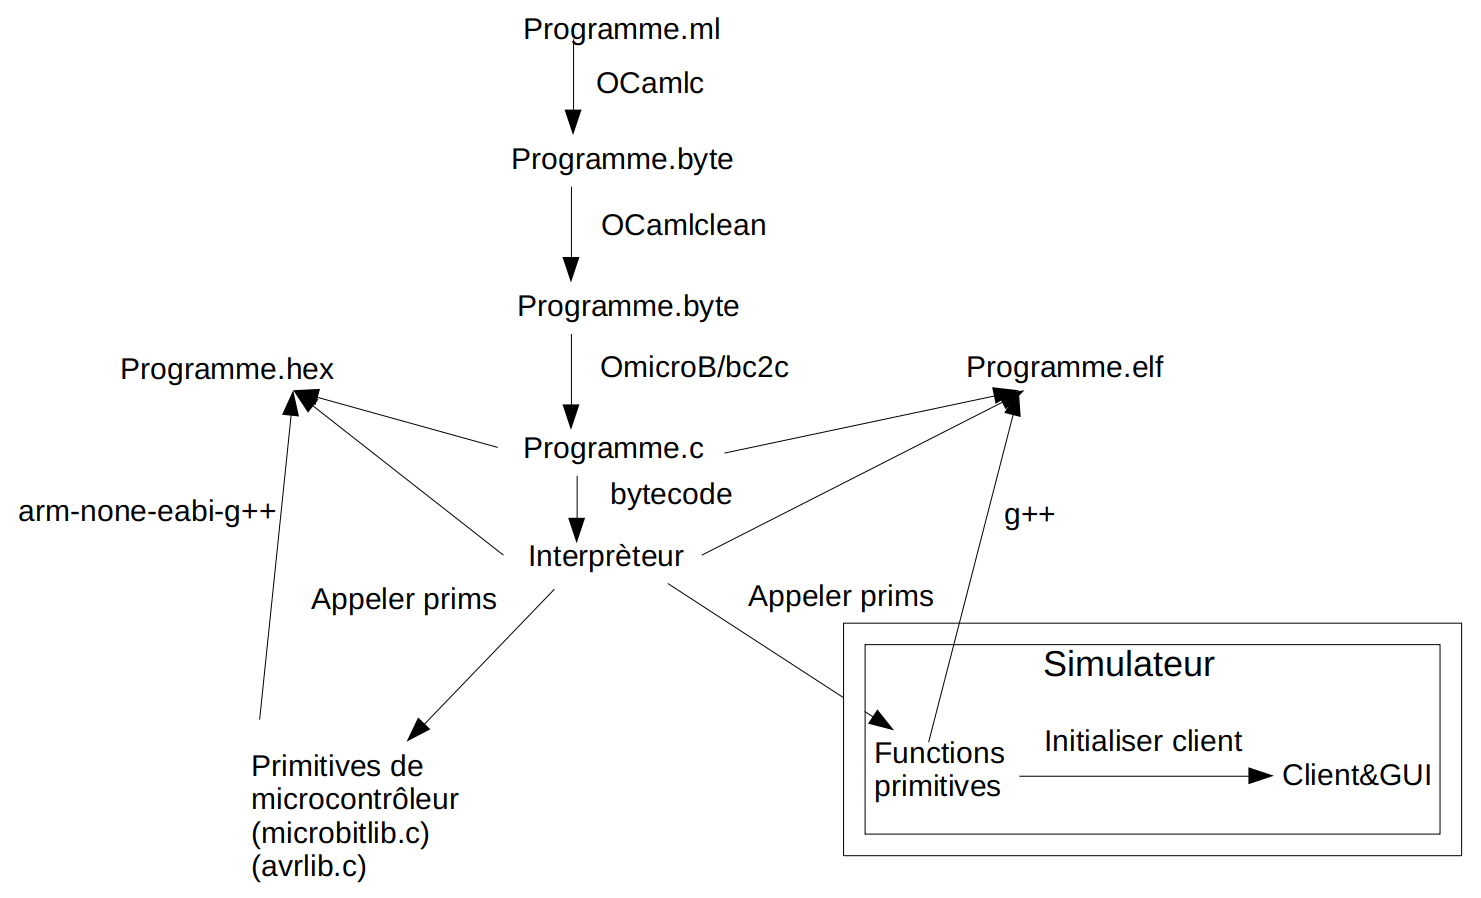
\includegraphics[width=0.8\textwidth]{StructureProgramme.png}
			\end{minipage}%
		}%
	\end{figure}
	
	Cette image montre chaque étape de compilation d'un programme OCaml par OMicroB.
	\begin{enumerate}
		\item \textbf{OCamlc} compile le fichier \textbf{.ml} avec la bibliothèque et génère un fichier \textbf{.byte}.
		\item \textbf{OCamlclean} traite le fichier généré \textbf{.byte}. L'outil OCamlclean qui transforme le bytecode OCaml pour supprimer les fermetures inutilisées du tas. Ce processus de nettoyage de bytecode est essentiel pour exécuter des programmes non triviaux sur des appareils avec un espace mémoire limité.[3]
		\item \textbf{bc2c} est le compilateur de \textbf{OMicroB}, il permet de transférer le code binaire à un programme \textbf{.c}. L'outil bc2c prend en entrée la sortie du fichier de bytecode par le linker OCaml OCamlc ou le nettoyeur de bytecode OCamlclean. Il effectue ensuite une analyse et des transformations de code pour optimiser et compacter le bytecode, et produit enfin un fichier source C définissant les constantes et les tableaux statiques nécessaires à l'implémentation OMicroB de la machine virtuelle OCaml décrite plus loin.[4]
		\item \textbf{g++} compile le \textbf{programme.c} et la bibliothèque de simulateur \textbf{sf-regs} puis génère le fichier exécutable \textbf{.elf}.
		\item \textbf{arm-none-eabi-g++} compile le \textbf{programme.c} avec la bibliothèque de microcontrôleur (avrlib, microbitlib, etc) puis génère le fichier exécutable \textbf{.hex}.
	\end{enumerate}
	
	\textbf{OMicroB} produit deux fichiers exécutables après la compilation d'un programme \textbf{OCaml}.\\
	- \textbf{.elf} est exécutable en mode simulation, il permet de démarrer le simulateur et montrer le changement des états de pin et les effets de programme sur une interface graphique.\\
	- \textbf{.hex} est exécutable sur Micro:bit comme l'effet fichier original OCaml exécuter sur Micro:bit.
	
	\subsection{Micro:bit}
	Le micro:bit est un microcontrôleur qu'on utilise beaucoup dans la vie, doté d'un processeur ARM. Conçu au Royaume-Uni pour un usage éducatif dans un premier temps, le nanoordinateur est maintenant disponible au grand public dans de nombreux pays.\\
	
	La taille de la carte de circuit est de 4 cm * 5 cm, avec un processeur ARM Cortex-M0, un capteur d'accélération et un capteur magnétique, des capacités de programmation de communication Bluetooth et de connexion USB, un écran composé de 25 LED, 2 boutons programmables, USB peut être utilisé Ou une batterie externe pour alimenter. L'entrée et la sortie de l'appareil comprennent des connecteurs à trous annulaires et des connecteurs latéraux.
	
	\subsubsection{Circuit de Micro:bit}
	Cette image montre le circuit du \textbf{microbit}, la matrice de LED se compose d'une matrice de pins de 3 * 9. Pour allumer un LED, on doit mettre le \textbf{pin\_row} correspondant au niveau \textbf{HIGH}, et mettre son \textbf{pin\_col} au niveau \textbf{LOW}.
	\begin{figure}
		\subfigure[cf.le circuit réel de microbit]{
			\begin{minipage}[t]{\linewidth}
				\centering
				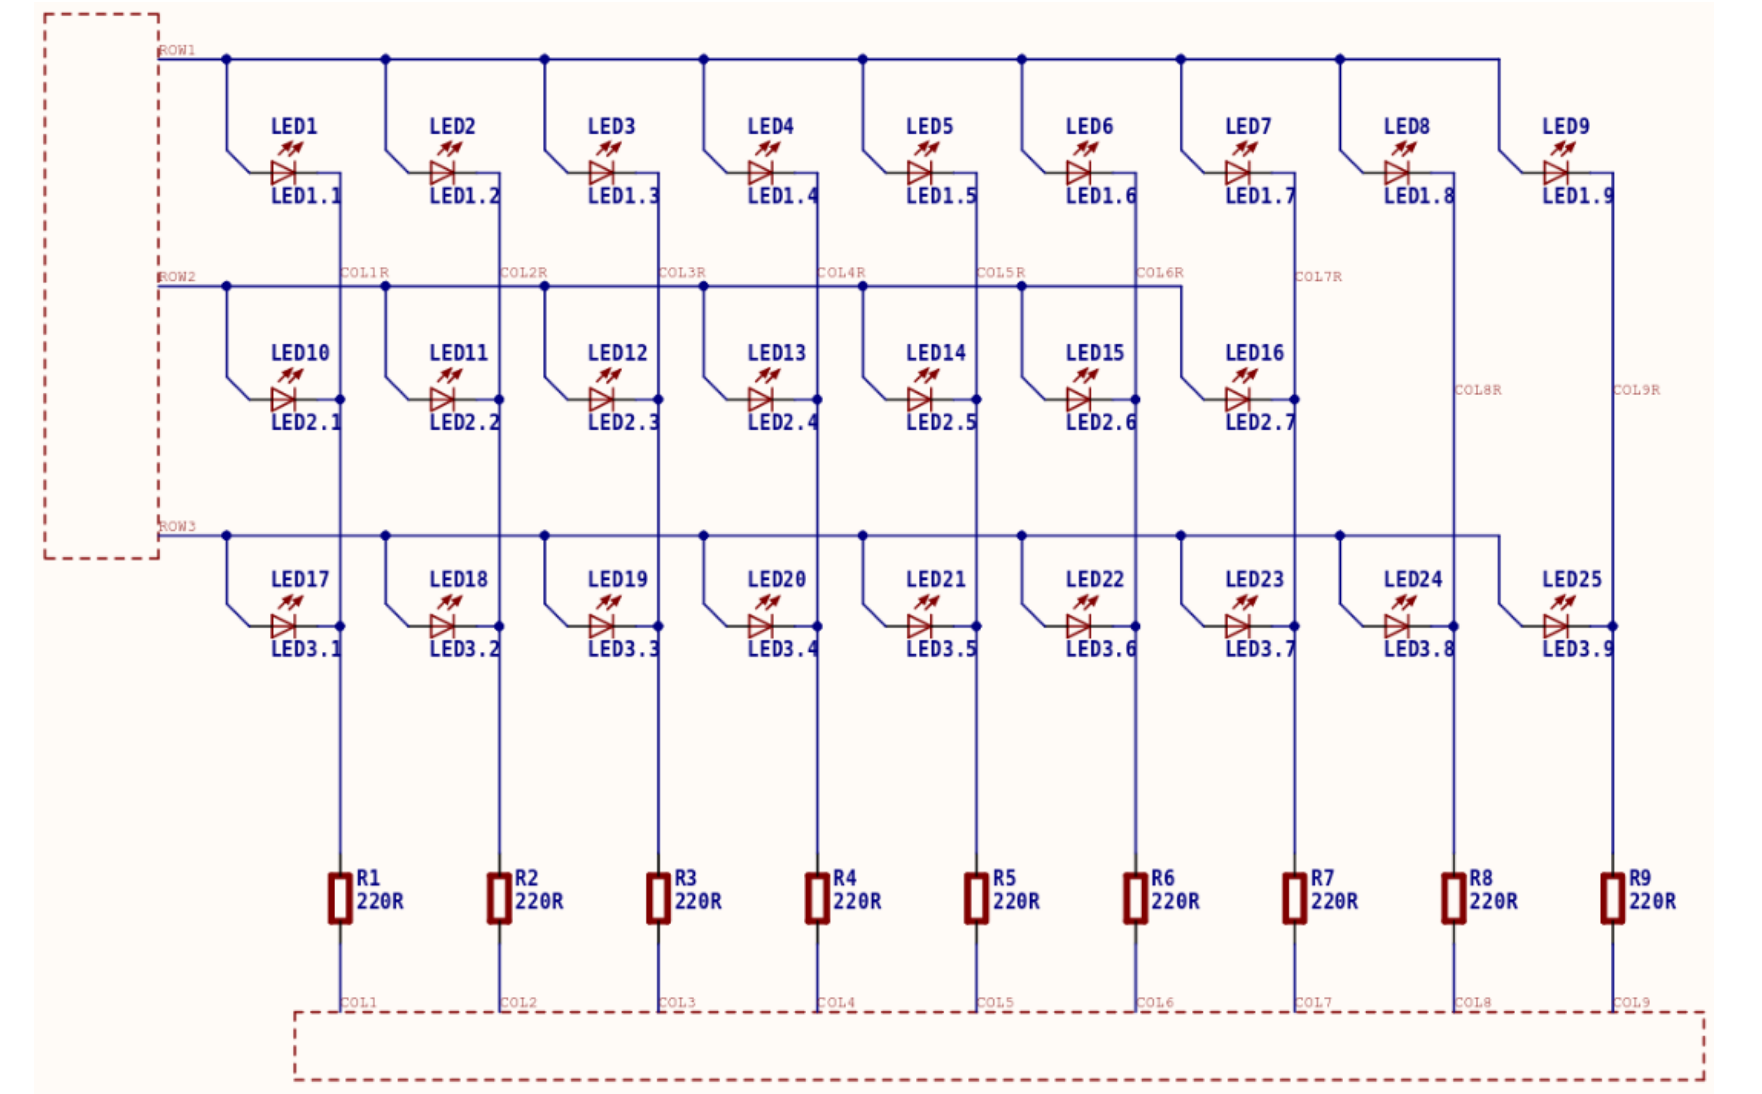
\includegraphics[width=0.8\textwidth]{circuitReelMicrobit.png}
			\end{minipage}%
		}%
	\end{figure}
	
	\clearpage
	Ce tableau montre la relation de position entre le circuit du \textbf{microbit} et l'écran du \textbf{microbit}.
	
	\begin{figure}
		\subfigure[le tableau des associations entre le LED et les pins correspondants]{
			\begin{minipage}[t]{\linewidth}
				\centering
				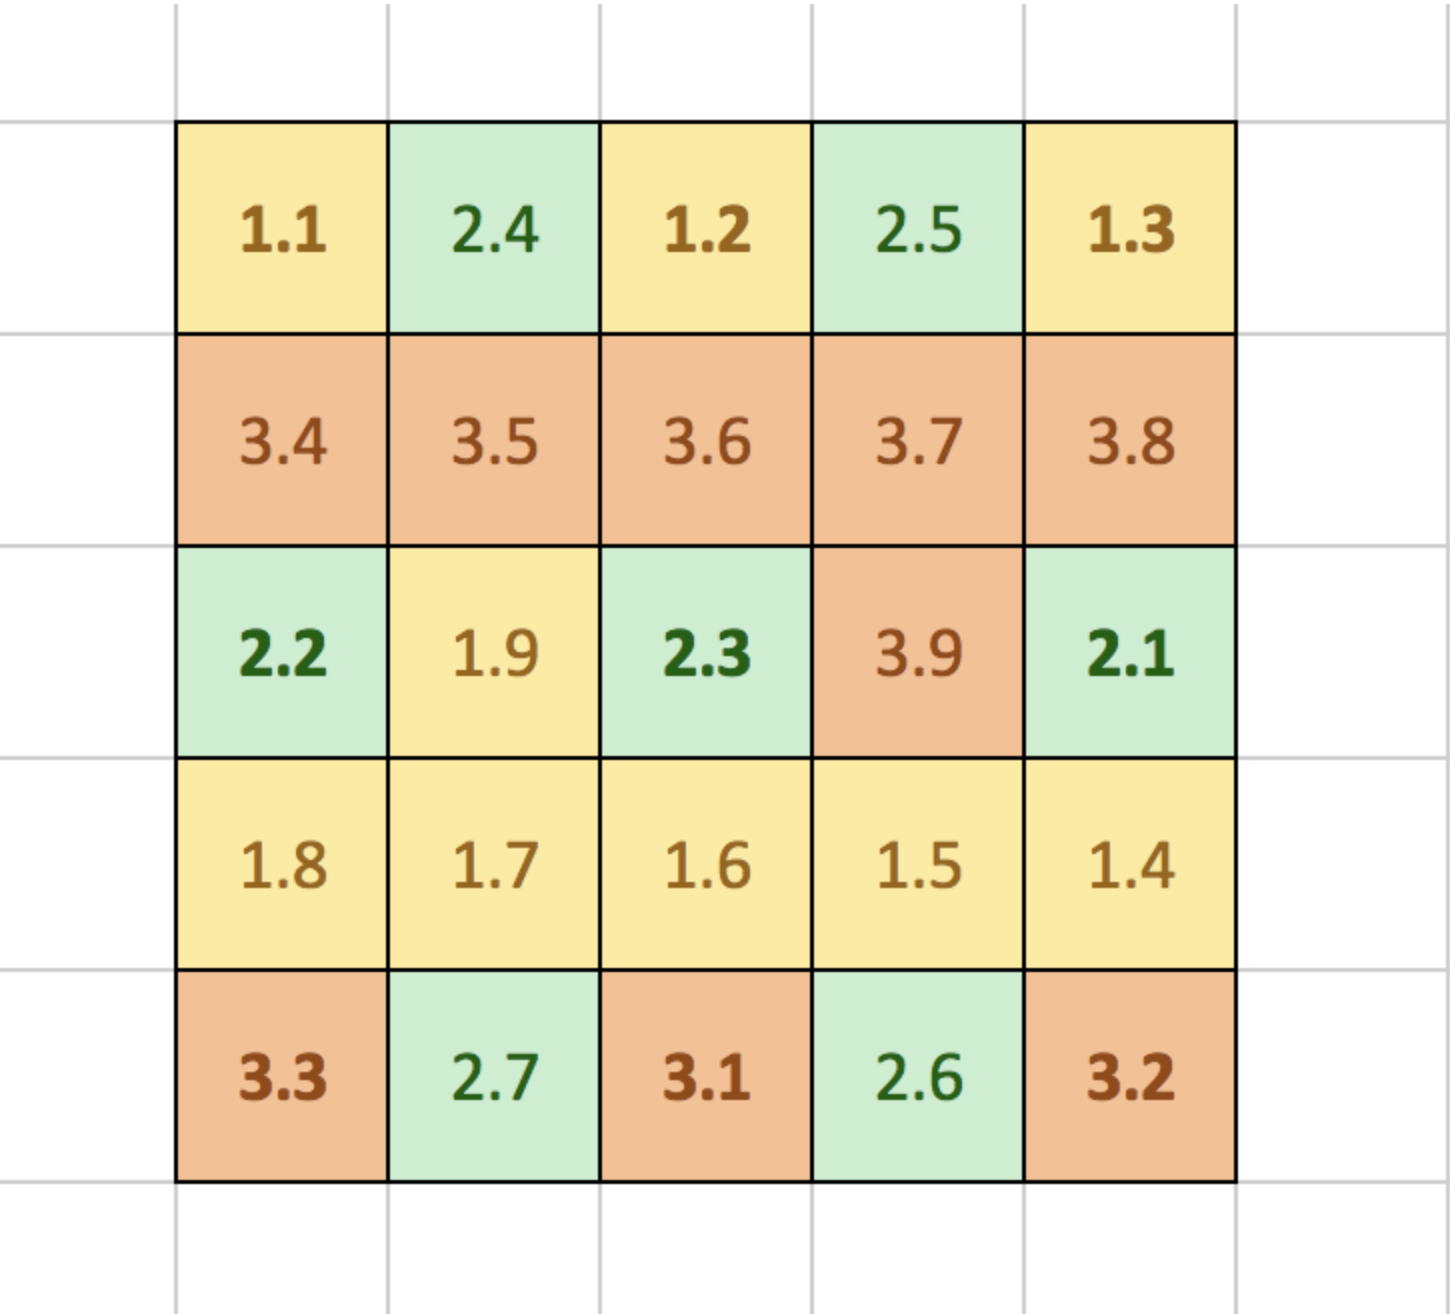
\includegraphics[width=0.3\textwidth]{matrice_Pins.png}
			\end{minipage}%
		}%
		
	\end{figure}
	
	\subsection{Problématique}
	Selon ce qui précède, même si omicrob peut déjà convertir des fichiers OCaml en fichiers hexadécimaux qui peuvent être exécutés sur le microcontrôleur, nous avons besoin d'un simulateur plus intuitif sur le PC pour simuler le comportement du microcontrôleur afin de faciliter l'utilisation du développement et de la programmation des programmeurs. Lors du développement de ce simulateur, nous devons penser à sa structure, comment utiliser le mécanisme de synchronisation, comment afficher visuellement l'effet du fichier converti par OmicroB etc. Dans manière générale, si l'architecture des différents microcontrôleurs est différente, le simulateur sera différent. Ce que nous voulons faire est un simulateur à usage général, qui peut être utilisé pour simuler une variété de Microcontrôleur, par exemple : Micro:bit, Arduino etc. Notre idée de développement est de faire d'abord un simulateur pour Micro:bit, puis on le rendre générique. C’est à dire qu'il pourra simuler une variété de microcontrôleurs et mettre en œuvre le montage.
	
	\clearpage
	\pagestyle{fancy}
	\lhead{Simulateur}
	\rhead{\thepage}
	\fancyfoot{}
	\section{Simulateur}
	Pour afficher les effets de programme exécuté sur un microcontrôleur, on propose un simulateur qui sert à afficher simultanément l'état de chaque pin et chaque composant pendant l'exécution du programme. Donc on peut considérer l'interpréteur de \textbf{OMicroB} comme un producteur qui produit les demandes de visualisation. Le simulateur est un consommateur, il satisfait chaque demande en visualisant les effets sur une interface graphique. Donc on peut implémenter une architecture \textbf{producteur-consommateur} pour réaliser le simulateur, un producteur transfère les demandes de l'interprèteur au consommateur, le consommateur visualise sur l'interface graphique finalement.\\
	
	Considérons la facilité du développement, nous séparons le simulateur en deux parties indépendantes, \textbf{serveur} et \textbf{client}, le serveur est producteur et client est consommateur. Ses avantages sont que :
	\begin{enumerate}
		\item Séparer le logiciel en deux parties indépendantes, nous pouvons développer paralèllement, c'est plus facile de travailler en groupe.
		\item On peut mieux maintenir le simulateur. Lorsqu'il y a des erreurs générées pendant l'exécution, il plus pratique de localiser où produit l'erreur.
	\end{enumerate}
	
	Par conséquence, on a un simulateur dont la structure est décrite par cette image, il exécute deux processus en concurrence. Chaque processus exécute plusieurs threads et travaillent asynchroniquement.
	
	\begin{figure}[htbp]
		\subfigure[la structure de simulateur]{
			\begin{minipage}[t]{\linewidth}
				\centering
				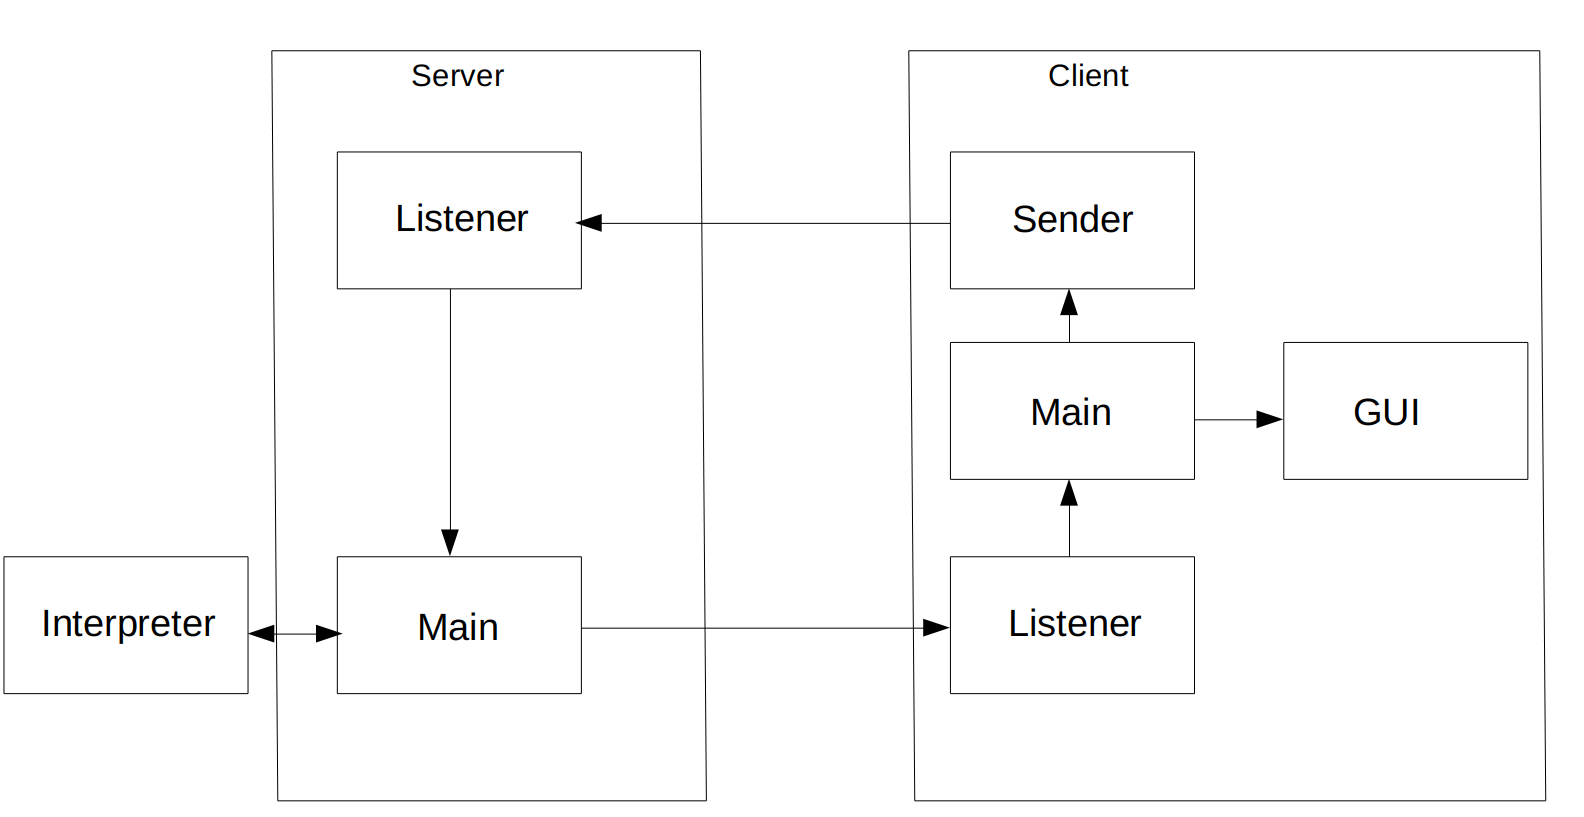
\includegraphics[width=\textwidth]{Simulator.png}
				%\caption{fig1}
			\end{minipage}%
		}%
	\end{figure}
	\subsection{Serveur}
	La partie serveur est codée en C dans "/src/byterun/", il contient des fichiers :
	\begin{enumerate}
		\item \textbf{/src/byterun/vm}.
		Ce dossier contient les fichiers de l'interprèteur d'OMicroB, il à été réalisé en OMicroB existant. Par exemple le format des type basiques de données, le garbage collector de machine virtuelle ainsi que les définitions des instructions de code binaire. Il exécute le programme OCaml et envoie les instructions au serveur.
		
		\item \textbf{/src/byterun/simul/sf-regs.c/.h}.
		C'est la bibliothèque des primitives de simulateur, le simulateur propose beaucoup d'API aux programmeurs d'OCaml. Ils peuvent appeler ces API dans un programme OCaml qui exécute sur un microcontrôleur, par exemple \textbf{set\_pixel 0 0 true} sert à allumer un LED de microbit. Lorsque ce API est utilisé, la fonction définie dans sf-regs.c est appelé. Elle envoie une instruction au client, puis le client allume LED sur l'interface graphique.
		
		\item \textbf{src/byterun/shared.c/.h}.
		Ce fichier définit des structures de données partagées entre le processus client et serveur, elles sont stockées dans une mémoire partagée au fur et mesure de l'exécution de programme.
	\end{enumerate}
	\textbf{Processus Serveur} exécute deux threads, \textbf{listener} et \textbf{Main}.
	\begin{enumerate}
		\item \textbf{Main} traite simplement l'instruction qui vient de l'interprèteur et l'envoyer au thread \textbf{listener} de client.
		\item \textbf{listener} reçoit l'instruction venant de \textbf{Sender} et informe \textbf{Main}.
	\end{enumerate}
	
	Dans cette partie, nous avons réalisé des primitives spécifiques de microbit et des primitives générales.
	\begin{enumerate}
		\item \textbf{microbit\_print\_char(char c)} sert à afficher une lettre sur l'écran 5x5 du microbit.
		Tout d'abord, nous convertissons les informations de tous les lettres en forme des graphiques raster dans une table en code hexadécimal 5x8 bits en bien tirer en ordre du code ASCII. Lorsqu'on recevoir une commande d'imprimer une lettre à l'écran,
		On va calculer ASCII code correspond à cette lettre, et puis en fonction de cet ASCII code, on peut calculer le décalage dans la table de code hexadécimal correspond à cette lettre. Sortir enfin les 5 * 8 bits d'information dont il dispose. Prendre 5 * 5 bits d'entre eux et les imprimer pixel par pixel sur l'écran.\\
		
		Un exemple de visualiser la caractère 'A' sur la matrice des leds.
		\begin{enumerate}
			\item calcule le code ASCII de 'A', c'est 65.
			\item calcule son décalage c'est 65 * 5 = 325. (Parce que l'écran est de 5 lignes et chaque ligne est composé de 2 chiffre hexadécimal)
			\item cherche son table de code hexadécimal correspondant dans le tableau, c'est \{30,28,38,28,28\}.
			\item nous convertissons code hexadécimal en forme code binaire.\\
			00110000\\
			00101000\\
			00111000\\
			00101000\\
			00101000
			\item modifier les Pins de chaque LED en fonction de cette code binaire. On a finalement une image comme cela.\\
			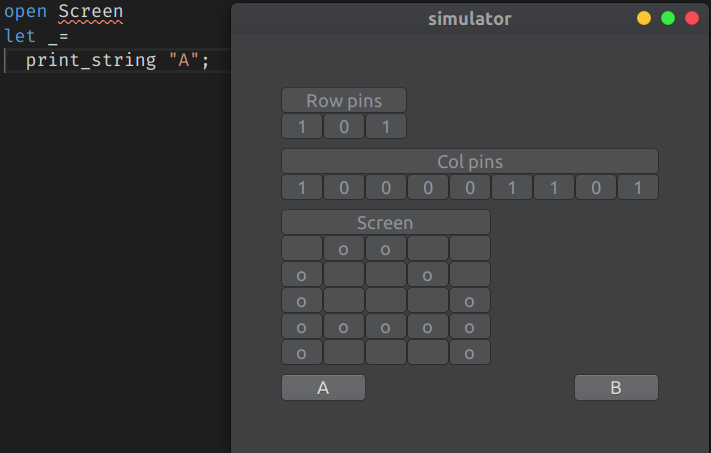
\includegraphics[width=0.6\textwidth]{printA.png}\\[1cm]
		\end{enumerate}
		
		\item \textbf{microbit\_print\_string(char *str)} permet d'afficher une chaine de caractères, une fois qu'on a réalisé la primitive \textbf{microbit\_print\_char(char c)}. Il ne suffit de parcourir cette chaine de caractère et appeler cette primitive pour chaque caractère.
		\item \textbf{microbit\_print\_int(int n)} sert à afficher un entier sur l'écran. On a juste besoin de formaliser cet entier en une chaine de caractères par \textbf{snprintf} et appeler \textbf{microbit\_print\_string(char *str)}.
		\item \textbf{void microbit\_write\_pixel(int col, int row, int l)} sert à mettre l'état du pixel dont coordonnées sur l'écran est (row, col) à l, si l’est 0, cela veut dire éteindre ce LED, sinon c'est allumer ce LED.
		\item \textbf{void microbit\_digital\_write(int p, int l)} permet de mettre l'état de pin p au niveau l (l=0 ou 1), si l=0, cela veut dire du niveau LOW, sinon c'est niveau HIGH.
		\item \textbf{int microbit\_digital\_read(int p)} sert à rendre le niveau de pin p.
		\item \textbf{void microbit\_analog\_write(int p, int l)} peut écrire une valeur sur le pin p, (0 <= l < 1024), cette primitive modifie le tableau pin\_val qui stocke les valeur des pins.
		\item \textbf{int microbit\_analog\_read(int p)} rend la valeur sur le pin p.
		\item \textbf{void microbit\_serial\_write(char c)} stocke la caractère c dans un buffer.
		\item \textbf{char microbit\_serial\_read()} lit un caractère depuis le buffer, puis le pointeur de tête incrémente 1.
		
		
	\end{enumerate}
	
	
	
	\subsection{Client}
	La partie client est programmée en C dans \textbf{src/byterun/client}, se compose de deux fichiers.
	\begin{enumerate}
		\item \textbf{client.c} définit les fonctions du travail par exemple traiter le message qui vient du côté serveur.
		
		\item \textbf{gui.c} implémente l'interface graphique par \textbf{gtk3.0}.
		il nous montre un UI de simulateur permet d'afficher le résultat de programme et les états des Pins pendant la simulation, ainsi que l'interaction par les boutons.\\
	\end{enumerate}
	
	\textbf{Processus Client} lance simultanément quatre threads, \textbf{Main}, \textbf{GUI}, \textbf{Sender} et \textbf{listener}.
	\begin{enumerate}
		\item \textbf{Main} est le premier thread principal, il traite les arguments venant de processus serveur et connecte aux mémoires partagés, par exemple la mémoire partagée pour la communication et pour le montage. Il est responsable d'exécuter les autres threads.
		\item \textbf{GUI} crée les composants de l'interface graphique en fonction de l'information du montage. Il actualise l'interface dans un boucle infini afin d'afficher le changement des états de chaque composant simultanément.
		\item \textbf{Sender} sert à traiter input de l'utilisateur et envoyer l'instruction au serveur, par exemple appuyer les boutons.
		\item \textbf{listener} reçoit l'instruction venant de serveur, en plus manipuler les composants de l'interface graphique en fonction de l'instruction.
	\end{enumerate}
	
	
	\pagestyle{fancy}
	\lhead{Mécanisme de communication}
	\rhead{\thepage}
	\fancyfoot{}
	
	\section{Mécanisme de communication}
	\subsection{Protocole de communication}
	Pour décrire bien l'instruction, on a implémenté le protocole en plusieurs versions diverses. (S -> C) représente la direction de l'envoie est du serveur au client, (C -> S) est la direction inversée.
	
	\subsubsection{Chaine de caractère}
	Dans la version de protocole initiale, Nous avons choisi la chaine de caractère comme le type du protocole. La raison est que c'est plus pratique de les afficher sur le terminal, on peut facilement vérifier si le protocole est correct pour chaque instruction. \\
	La structure du protocole est (\textbf{numéro de primitive, argument1, argument2, .....}).
	Pour cette version, nous avons réalisé les protocoles.
	\begin{enumerate}
		\item \textbf{PRINT\_IMAGE}: (0, 25 caractères de 0 ou 1)\\
		(S -> C) Il sert à afficher une image en fonction de 25 caractères, chaque caractère représente l'état de LED. Envoyé par \textbf{microbit\_print\_image(char* ima)}.
		\item[-] \textbf{SET\_PIXEL(x,y,val)}: (1, x, y, val)\\
		(S -> C) Modifier l'état du pixel des coordonnées x et y à val, envoyé par \textbf{microbit\_write\_pixel(int x, int y, int val)}.
		\item[-] \textbf{CLEAR\_SCREEN}: (2)\\
		(S -> C) Mettre les états de tous les pixels à 0, envoyé par \textbf{microbit\_clean\_screen()}.
		\item[-] \textbf{SET\_PIN(p,n)}: (3, numéro de pin, niveau)\\
		(S -> C) Modifier le pin p au niveau n. (n = 0 ou 1), envoyé par \textbf{microbit\_digital\_write}.
		\item[-] \textbf{WRITE\_PIN(p,v)}: (5, p, v)\\
		(S -> C) Modifier le pin p à la valeur v (0 <= v <= 1024), envoyé par \textbf{microbit\_analog\_write}.\\
		
		\item[-] \textbf{INVERSE\_PIN(p,n)}: (0, p)\\
		(C -> S) Inverser l'état de pin qui associe avec un bouton, lorsque l'utilisateur appuie sur un bouton, ce protocole est envoyé au serveur et \textbf{serveur listener} inverse l'état de pin correspondant.
	\end{enumerate}
	
	\subsubsection{Entier de 32 bits}
	Après tester toutes les primitives, on est sûr que le protocole a correctement décrit chaque instruction. On commence d'améliorer ce protocole, parce que la formalisation et décodage du protocole consomment beaucoup de temps, ainsi que la chaine de caractère consomment aussi l'espace de mémoire.\\
	Comme un integer du langage C se compose de 32 bits, ainsi que 32 bits pour le protocole est suffisant sauf pour PRINT\_IMAGE. Il ne suffit pas à afficher une image dont le nombre de pixel est supérieur à 31. Donc on supprime ce protocole dans cette version, et on réalise la primitive \textbf{microbit\_print\_image(char* ima)} en utilisant le protocole \textbf{SET\_PIXEL(x,y,val)}, il ne suffit d'envoyer le nombre de pixel fois le protocole \textbf{SET\_PIXEL(x,y,val)}.
	
	Par conséquence, la structure du nouveau protocole est \textbf{(numéro de méthode 7bits) :: arguments(25 bits)}.\\
	7 bits pour le numéro de fonction, on peut étendre jusqu'à 128 primitives maximum, c'est très suffisant. \\ 25 bits suffit de représenter tous les arguments pour l'instant.
	Il y à des protocoles comme ci-dessous
	\begin{enumerate}
		\item[-] \textbf{SET\_PIXEL(x,y,val)}: 1(7bits)::x(12 bits)::y(12 bits)::val(1 bits), (S -> C)
		\item[-] \textbf{CLEAR\_SCREEN}: 2(32 bits), (S -> C)
		\item[-] \textbf{SET\_PIN(p,n)}: 3(7 bits)::p(8 bits)::n(17 bits), (S -> C)
		\item[-] \textbf{WRITE\_PIN(p,v)}: 4(7 bits)::p(8 bits)::v(17 bits), (S -> C).\\
		
		\item[-] \textbf{INVERSE\_PIN(p,n)}: 0(7 bits)::p(25 bits) (C->S).
	\end{enumerate}
	
	
	\subsection{Synchronization}
	Deux processus exécutent en concurrence, le plus important est que comment synchroniser leur tâche ? Nous avons testé le simulateur sans synchronisation, et nous avons observé qu'il y a des protocoles qui ne sont pas visualisées sur l'interface graphique. C'est parce que la visualisation de quelques protocoles prend du temps. Par exemple éteindre tous les LEDs ou afficher une image. Donc on a implémenté un mécanisme de communication, il sert à garantir que chaque protocole peut être bien visualisée. Ce sont les étapes pour la communication entre le processus serveur et client.
	
	\textbf{Etapes pour afficher d'un protocole}
	\begin{enumerate}
		\item \textbf{Client listener} attend le protocole de serveur.
		\item \textbf{Server main} vérifie si le protocole précédente est bien visualisé.\\
		- Si oui, il envoie le nouveau protocole au client.\\
		- Sinon, \textbf{Server main} attend .
		\item \textbf{Server main} réveille le thread \textbf{client listener}.
		\item \textbf{Client listener} vérifie si la nouvelle instruction arrive.\\
		- Si oui, il informe au \textbf{GUI} afin d'afficher le nouvel état de composant.\\
		- Sinon, c'est un déblocage faux, il continue à attendre.
		\item \textbf{Client listener} réveille le thread \textbf{server main}.
		\item retour à l'étape 1.
	\end{enumerate}
	
	Pour garantir que ces deux processus exécutent étape par étape. Nous avons essayé plusieurs manières diverses au fur et mesure du développement.
	
	\subsubsection{Pipe + Signal}
	Au début, nous utilisions la pipe et le signal pour transmettre l'instruction. Pour la direction du serveur au client, le protocole est transmis par la pipe, et la direction inverse, on a utilisé le signal pour représenter le protocole, parce qu'il n'y a que événements, soit appuyer le bouton A soit le bouton B, donc on a attaché deux signaux SIGUSR1 et SIGUSR2 au ces deux bouttons, si le bouton est appuyé, le serveur reçoit SIGUSR1 ou SIGUSR2, et la fonction \textbf{handler} inverse l'état de pin correspondant.
	
	Son avantage est que l'on n'a plus besoin exécuter un thread \textbf{listener} dans le processus \textbf{serveur}. Comme la fonction \textbf{handler} exécute dès que le processus serveur reçoit le signal depuis le processus client.
	
	Mais le mécanisme de signal est très limité, le signal utilisable est divers pour le système différent, par exemple pour linux on a droit d'utiliser les signaux qui sont supérieur à 32, mais pour macOS, il y a seulement quatre signaux qu'on peut utiliser.
	
	\subsubsection{Pipes}
	Après qu'on a constaté la limite du signal, on a essayé d'utiliser deux pipes pour la communication en deux directions. Pipe possède le mécanisme de protection, et il peut synchroniser automatiquement la communication, mais il 	génère un fichier temporaire pour la lecture et l'écriture, ainsi qu’il est moins efficace que la mémoire partagée. Donc on a finalement décidé d'utiliser la mémoire partagée.
	
	\subsubsection{Mémoire partagée}
	La mémoire partagée sert à communiquer entre le serveur et client, puisque c'est la plus rapide manière du transport de données. Mais son inconvénient est que l'on doit implémenter un mécanisme de synchronisation afin de protéger les données partagées pour la lecture et l'écriture. Donc pour deux directions du transport (du serveur au client et du client au serveur), on a besoin de deux mémoires partagées, \textbf{shm1} est écrit par le serveur, le client le lit. \textbf{shm2} est inversé.\\
	
	Afin de synchroniser la lecture et l'écriture, on met un mutex et une variable conditionnelle pour chaque mémoire partagée. Il garant que chaque instruction de serveur peut être bien traiter.\\
	
	
	
	
	\clearpage
	\pagestyle{fancy}
	\lhead{Méthodologie de réalisation}
	\rhead{\thepage}
	\fancyfoot{}
	
	\section{Méthodologie de réalisation}
	Selon ce qui précède, notre objectif est de simuler les informations d'entrée et de sortie du microcontrôleur, pour réaliser les fonctionnalité du simulateur, il y a deux versions, en \textbf{haut niveau} et en \textbf{bas niveau}.
	
	\subsection{Version haut niveau}
	\textbf{Haut niveau} est que l'on simule abstraitement un microcontrôleur, la simulation haut niveau ne reflète pas les interactions réelles entre le microcontrôleur et son environnement. On implémente les tableaux pour stocker les états de chaque composant. Dès que l'état de composant est modifié par la primitive, on modifie le tableau directement.\\
	Par exemple le serveur appelle la primitive \textbf{microbit\_write\_pixel 0 0 true}, il ne suffit de modifier le tableau qui stock l'état des LEDs. pixels[0][0] = true.\\
	
	\textbf{Avantage}\\
	La version est plus simple, il a juste besoin de modifier le tableau correspondant.\\
	
	\textbf{Inconvénient}\\
	Cette méthode n'est pas générale, parce que les composants sont différents pour les microcontrôleurs divers, on ne peut pas implémenter les tableaux pour chaque microcontrôleur.
	Si le microcontrôleur se change, nous devons réimplémenter le protocole et les tableaux des composants.
	
	
	\subsection{Version bas niveau}
	\textbf{Bas niveau} est que l'on simule réellement un microcontrôleur, afin de mieux simuler l'état de fonctionnement réel du microcontrôleur à partir de l'architecture du microcontrôleur, nous espérons modifier directement l'état du \textbf{tableau de pins}, sans avoir besoin d'autres appels de fonctions, et refléter directement les effets de ces modifications sur \textbf{l'interface graphique}. Cela fera quelques changements basés sur le haut niveau précédent.
	
	Lorsque nous voulons allumer un led, nous devons d'abord chercher son \textbf{pin} correspondant, puis mettons ce \textbf{pin} à haut niveau.\\
	
	\textbf{Avantage}
	Le simulateur de bas niveau peut s'adapter à un grand nombre de composants électroniques externes au microcontrôleur puisque les interactions sont réalisées par la modification des états des pins. Donc le protocole \textbf{SET\_PIN} est général pour le plupart des primitives, on n'a plus besoin de protocole spécifique comme \textbf{SET\_PIXEL}. Même si le microcontrôleur branche un composant spécifique, par exemple le moteur, l'écran LCD, etc., on a juste besoin de changer un fichier du montage, et rajouter un protocole spécifique mais pas tout le simulateur.\\
	
	\textbf{Inconvénient}
	Le traitement d'une instruction est plus compliqué, l'interaction entre le serveur et le client est plus fréquente.\\
	Par exemple, pour allumer un \textbf{LED} du microbit, le serveur envoie une seule instruction \textbf{SET\_PIXEL(X,Y,True)} au client dans la version haut niveau. Mais dans le bas niveau, comme on a présenté au début, il est contrôlé par deux pins, le serveur doit d'abord chercher le \textbf{pin\_row} et \textbf{pin\_col}, puis envoyer deux instructions \textbf{SET\_PIN(pin\_row, 1)} et \textbf{SET\_PIN(pin\_col, 0)} au client.
	
	\clearpage
	\pagestyle{fancy}
	\lhead{Montage}
	\rhead{\thepage}
	\fancyfoot{}
	
	\section{Montage}
	Pour réaliser un simulateur plus général, il doit supporter le montage. Cela veut dire que l'utilisateur peut ajouter les composants électronique externe comme il veut. Il peut décrire les paramètres du composant, soit des LEDs, soit des boutons, ainsi que les pins correspondants dans un fichier \textbf{circuit.txt}. Lorsque la première fois d'appeler la primitive, le simulateur est initialisé, un processus montage est exécuté par le processus serveur, il analyse \textbf{circuit.txt} par \textbf{lexer} et \textbf{parser}, ainsi que faire l'analyse sémantique pour évaluer ce fichier. Après l'évaluation, une structure qui stocke les informations du montage est transférée au processus client. Et le client peut recevoir les informations des composants du microcontrôleur depuis cette mémoire partagée, puis implémenter l'interface graphique selon ces informations.
	
	Cette fonctionnalité est réalisée dans le dossier \textbf{src/byterun/montage}, la structure est définie dans \textbf{src/byterun/simul/share.h}.
	
	\subsection{Analyser le ficher du montage}
	Pour le montage de microcontrôleur, il a besoin d'un fichier qui stocke les informations de chaque composant de microcontrôleur comme le nombre des pins, les associations entre chaque composant et le pin correspondant. Une fois que le simulateur connait ces informations, il peut implémenter l'interface graphique et contrôler les composants par modifier l'état des pins.\\
	Donc on a utilisé Flex, Yacc et langage C afin de réaliser un langage descriptif.
	\begin{enumerate}
		\item On définit les \textbf{tokens} dans le fichier \textbf{parser.y}.
		\item Lier les mots prédéfinis avec ces tokens dans \textbf{lexer.lex}
		\item Créer les nœuds de \textbf{AST}(l'arbre d'analyse syntaxe) dans fichier \textbf{AST.c} et \textbf{AST.h}.
		\item Réaliser les fonctions de l'évaluation dans le fichier \textbf{montage.c}.
	\end{enumerate}
	
	\begin{figure}[htbp]
		\subfigure[cf.exmple \textbf{circuit.txt}]{
			\begin{minipage}[t]{\linewidth}
				\centering
				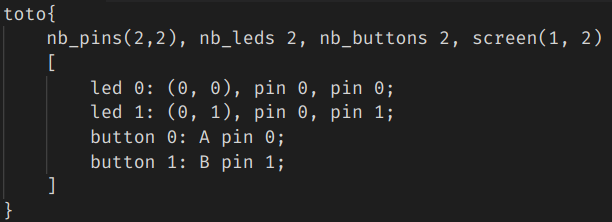
\includegraphics[width=0.5\textwidth]{circuit_ex.png}\\[1cm]
				%\caption{fig1}
			\end{minipage}%
		}%
	\end{figure}
	
	\textbf{Le grammaire et les mots prédéfinis}
	\begin{enumerate}
		\item \textbf{nom du simulateur\{l'information du montage\}}: C'est la structure du langage.
		\item \textbf{nb\_pins (num\_row, num\_col)}: \textbf{num\_row} est le nombre de pins de ligne(row), \textbf{num\_col} est celui de colonne.
		\item \textbf{nb\_leds num}: \textbf{num} est le nombre de leds.
		\item \textbf{nb\_buttons num}: \textbf{num} est le nombre de buttons.
		\item \textbf{screen(row, col)}: Cela indique le nombre de ligne et colonne de l'écran, par exemple si on veut un écran 5x5, on met screen(5, 5).
		\item \textbf{led id: (row, col), pin id1, pin id2}: Cela représente le numéro du LED et ses coordonnées sur l'écran, ainsi que l'association entre le led et deux pins correspondant. id1 est l'identifiant de pin row, id2 est celui de pin col.
		\item \textbf{button id: étiquette pin id}: Cette une déclaration du bouton dont l'identifiant est id et son étiquette, ainsi que le pin correspondant.
	\end{enumerate}
	Le nombre total de chaque composant est utilisé pour que le processus client alloue un tableau qui stocke les informations par \textbf{malloc}.
	
	
	\clearpage
	\pagestyle{fancy}
	\lhead{Méthodologie de réalisation}
	\rhead{\thepage}
	\fancyfoot{}
	
	\clearpage
	
	
	
	\section{Scénarios et Tests}
	Ce sont les étapes de simuler un programme ocaml par le simulateur du microbit.
	\begin{enumerate}
		\item Charger l'information du montage par un fichier \textbf{circuit.txt}.
		\item Le processus montage analyse ce fichier et génère une structure du montage, en plus envoie au serveur et au client par le mémoire partagée \textbf{envid}.
		\item Le processus client implémente une interface graphique en fonction de structure du montage.
		\item Le processus serveur alloue un tableau pour stocker les états de chaque pins par \textbf{malloc} en fonction de l'information du montage.
		\begin{figure}[htbp]
			\centering
			\subfigure[la description du circuit]{
				\begin{minipage}[t]{0.35\linewidth}
					\centering
					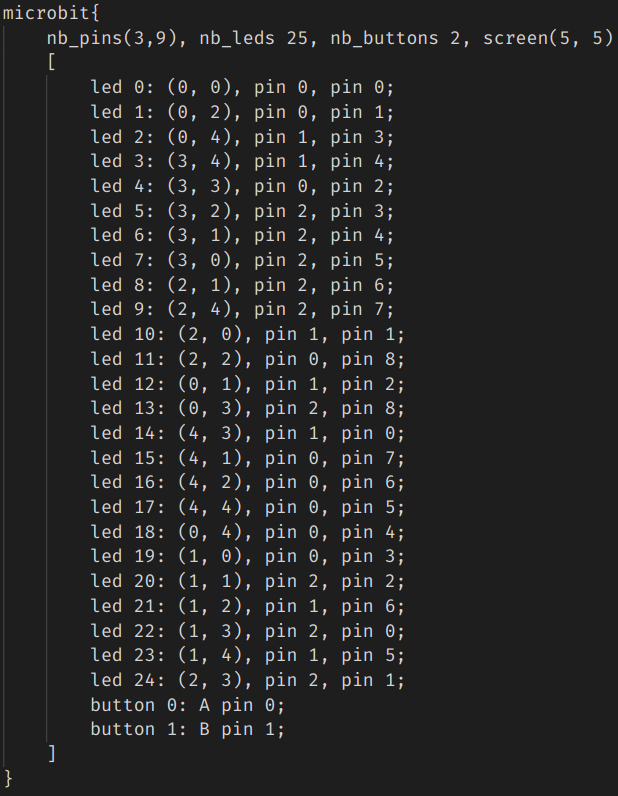
\includegraphics[width=\textwidth]{circuit.png}
				\end{minipage}%
			}%
			\subfigure[l'interface graphique de microbit]{
				\begin{minipage}[t]{0.4\linewidth}
					\centering
					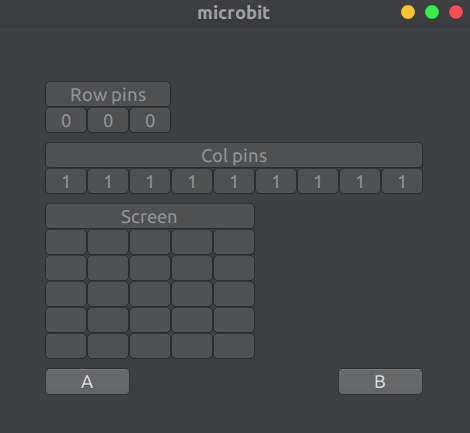
\includegraphics[width=\textwidth]{gui.png}
				\end{minipage}%
			}%
			\centering
		\end{figure}
		\item Le serveur interprète le programme OCaml, puis envoie des messages qui suivent le protocole au client.
		\item Le client affiche les effets du programme.
		\begin{figure}[htbp]
			\centering
			\subfigure[un programme ocaml]{
				\begin{minipage}[t]{0.4\linewidth}
					\centering
					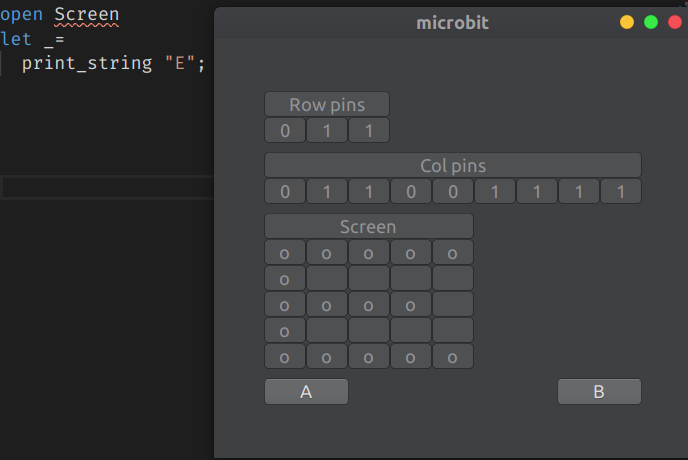
\includegraphics[width=\textwidth]{printE.png}
				\end{minipage}%
			}%
		\end{figure}
		
	\end{enumerate}
	\clearpage
	
	\section{Problème et Solution}
	\subsection{Problème de conflit pour micro:bit}
	Lorsque nous voulons allumer un seulement LED sur un micro:bit, il n'y a pas de conflit. Par exemple, pour \textbf{LED 0 0}, on met \textbf{pin\_row1} au niveau \textbf{HIGH}, et \textbf{pin\_col1} au niveau \textbf{LOW}. Les effets de la simulation est comme cet image.\\
	\begin{figure}[htbp]
		\subfigure[cf.exmple \textbf{allumer LED 0 0}]{
			\begin{minipage}[t]{\linewidth}
				\centering
				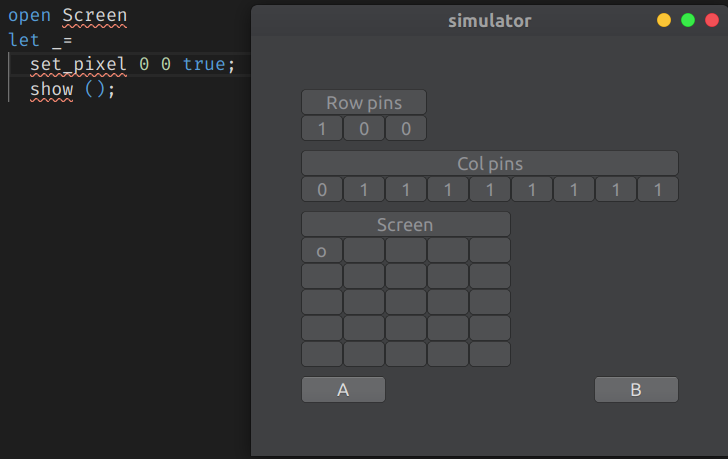
\includegraphics[width=0.45\textwidth]{no-conflict.png}\\[1cm]
				%\caption{fig1}
			\end{minipage}%
		}%
	\end{figure}\\
	
	Néanmoins, si on veut allumer deux LEDs dont le pin\_row n'est pas la même, il y aura le conflit. Par exemple on allume \textbf{LED 0 0} et \textbf{LED 0 1}. On doit mettre \textbf{pin\_row1} et \textbf{pin\_row3} au niveau \textbf{HIGH}, mettre \textbf{pin\_col1} et \textbf{pin\_col4} au niveau \textbf{LOW}. Dans ce cas-là, il y aura quatre LEDs allumé.
	\begin{enumerate}
		\item \textbf{LED 0 0} correspond à \textbf{pin\_row1, pin\_col1}.
		\item \textbf{LED 4 3} correspond à \textbf{pin\_row1, pin\_col4}.
		\item \textbf{LED 0 1} correspond à \textbf{pin\_row3, pin\_col4}.
		\item \textbf{LED 2 4} correspond à \textbf{pin\_row3, pin\_col1}.
	\end{enumerate}
	\begin{figure}[htbp]
		\subfigure[cf.exmple \textbf{allumer LED 0 0 et LED 0 1}]{
			\begin{minipage}[t]{\linewidth}
				\centering
				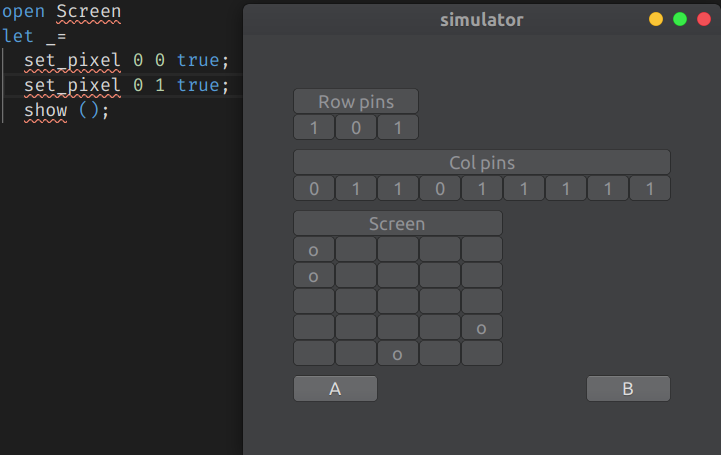
\includegraphics[width=0.45\textwidth]{conflit.png}\\[1cm]
				%\caption{fig1}
			\end{minipage}%
		}%
	\end{figure}
	
	Pour résoudre ce problème, on a ajouté une primitive \textbf{show ()} dans la bibliothèque de micro:bit et aussi dans la bibliothèque du simulateur sf-regs.c. Lorsque l'on appelle show (). On fait les étapes suivantes.
	\begin{enumerate}
		\item Chercher les pixels qu'on veut allumer dont le pin\_row est le pin\_row1.
		\item Mettre le pin\_row1 au niveau HIGH et les pin\_cols de ces pixels au niveau LOW.
		\item Allumer tous les pixels dont le pin\_row est pin\_row1.
		\item Éteindre ces pixels allumés, recouvrer les états des pins.
		\item Traiter la ligne suivante.
	\end{enumerate}
	On allume les pixels ligne par ligne, les pixels dont le pin\_row divers clignote très vite, pour avoir un effet d'allumer tous les pixels en même temps sans conflit.
	
	
	
	\section{Conclusion}
	Ce projet nous a permis de découvrir le domaine du microcontrôleur qui était obscur pour nous. Nous avons appris les caractéristiques et l'architecture du microcontrôleur et exploré les aspects de développement en fonction des restrictions du microcontrôleur.
	
	Nous avons aussi appliqué ce que nous avons appris lors du master 1 en cours de "Développement d'un langage de programmation", et en "Analyse des programmes et sémantique".
	
	Nous avons réalisé les fonctions de base du simulateur. L’interaction entre le client et le serveur du simulateur est stable, et il peut simuler l'effet du fichier OCaml compilé par OmicroB exécuté sur Micro:bit.
	
	Malheureusement, comme nous l'avons exprimé précédemment, nous n'avons pas le temps d'enrichir les fonctions du simulateur et de le tester sur des microcontrôleurs Arduino. Bien que nous ayons passé beaucoup de temps à essayer différentes méthodes pour implémenter le simulateur, nous pensons que ces tentatives ne sont pas uniquement pour ce projet. Il a également accumulé de l'expérience sur notre future de programmation.
	
	\section{Références}
	[1]Matt Oppenheim,"Measuring the BBC micro:bit LED current draw",2019,[Online].\\
	Available:https://www.seismicmatt.com/2019/03/06/measuring-the-bbc-microbit-led-current-draw/\\
	
	[2]Micro:bit,"Micro Bit Light Sensor",[Online].\\
	Available:https://lancaster-university.github.io/microbit-docs/extras/light-sensing/\\
	
	[3][4]Steven Varoumas, Benoît Vaugon, Emmanuel Chailloux."A Generic Virtual Machine Approach for Programming Microcontrollers: the OMicroB Project",Toulouse, France.[Online].\\
	Available:https://hal.sorbonne-universite.fr/hal-01705825/document\\
	
	
\end{document}